\documentclass{article}
\usepackage[utf8]{inputenc}
\usepackage{graphicx}
\usepackage{amsthm}
\usepackage{amsmath}
\usepackage{amssymb}
\usepackage{amsfonts}
\usepackage{color}
\usepackage{wrapfig}
\usepackage[francais]{babel}
\usepackage{fancyvrb}
\usepackage{hyperref}

\title{TP4\\ Arithmétique}
\author{BRAHMI Kahina et HARDY Marion}

\begin{document}
\maketitle


\section{EXERCICE : Un nombre est-il premier}

	Tout d'abord nous avons cherché comment obtient en python le quotient et le reste de la dividion euclidienne d'un entier par un autre entier. 
\\

On a explicité la definition d'un nombre premier; un nombre premier étant un nombre divisible que par 1 ou par lui même.
\\

Aussi on a identifié les nombres premiers de la liste suivante : 1001, 2017, 3001, 49999, 89999, qui se trouve être : 2017, 3001, et 49999.
\\

Ensuite nous avons defini la fonction \textbf{ is\_prime} qui prend en argument un entier $n$ et renvoie {\bf true} si $n$ est premier et {\bf false} si $n$ n'est pas premier.\\
On a également pu determiné si les nombres Fermat $F_{n}$ étaient des nombres premiers à l'aide de la fonction \textbf{ is\_prime}.


\section{EXERCICE : Crible d'Erasthotène}

La crible d'Erasthotène nous a permis de calculer la liste de tous les nombres premiers inférieurs à 200. (voir annexe)
\\

En effet, nous avons défini une fonction python qui donne tout les nombres premiers jusqu'à un certain $n$.\\
Cette fonction nommé {\bf primes} prend en argument un entier $n$ et renvoie la liste de tous les nombres premiers inférieurs à cet entier $n$.
\\

Puis nous avons testé la fonction {\bf primes} en posant $n$=1000 ce qui nous a permis de calculer la liste de tous les nombres premiers inférieurs à 1000. Nous avons reporté ces nombres premiers dans un fichier nommé {\bf primes.txt}.
\\

Ensuite on a représenté graphiquement la fonction $\pi(n)$ et la fonction $\dfrac{n}{\log n}$ avec $n$ allant de 2 à 1000. On a donc pu observer que les deux fonctions étaient presque équivalente.\\ Autrement dis on peut utilisé la fonction $\dfrac{n}{\log n}$ comme approximation de la fonction $\pi(n)$.

\begin{center}
	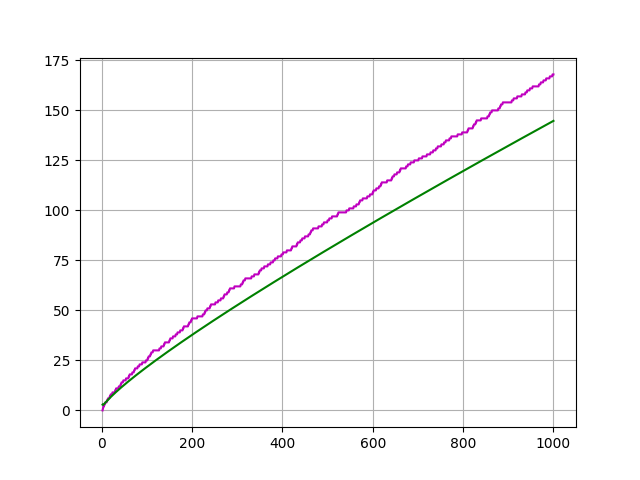
\includegraphics[scale=0.5]{graph1.png}
\end{center}
 
Aussi on a pu remplir le tableau suivant :

\begin{center}
\begin{tabular}{r | c | c}
$n$ & $\pi(n)$ & $\frac{n}{\log n}$ \\
\hline
$10^1$ & {4} & {4.34294481903}\\
$10^2$ & {25} & {21.7147240952}\\
$10^3$ & {168} & {144.764827301}\\
$10^4$ & {1229} & {1085.73620476}\\
$10^5$ & {9592} & {8685.88963807}\\
$10^6$ & {} & {}
\end{tabular}
\end{center}

\section{EXERCICE : Factorisation d'un entier premiers}






























\end{document}

